\documentclass[14pt]{extbook}
\usepackage{multicol, enumerate, enumitem, hyperref, color, soul, setspace, parskip, fancyhdr} %General Packages
\usepackage{amssymb, amsthm, amsmath, latexsym, units, mathtools} %Math Packages
\everymath{\displaystyle} %All math in Display Style
% Packages with additional options
\usepackage[headsep=0.5cm,headheight=12pt, left=1 in,right= 1 in,top= 1 in,bottom= 1 in]{geometry}
\usepackage[usenames,dvipsnames]{xcolor}
\usepackage{dashrule}  % Package to use the command below to create lines between items
\newcommand{\litem}[1]{\item#1\hspace*{-1cm}\rule{\textwidth}{0.4pt}}
\pagestyle{fancy}
\lhead{Progress Quiz 5}
\chead{}
\rhead{Version B}
\lfoot{8497-6012}
\cfoot{}
\rfoot{Summer C 2021}
\begin{document}

\begin{enumerate}
\litem{
Solve the quadratic equation below. Then, choose the intervals that the solutions belong to, with $x_1 \leq x_2$ (if they exist).\[ 17x^{2} +14 x -5 = 0 \]\begin{enumerate}[label=\Alph*.]
\item \( x_1 \in [-0.4, -0.1] \text{ and } x_2 \in [0.71, 1.59] \)
\item \( x_1 \in [-23.6, -21.9] \text{ and } x_2 \in [22.69, 23.43] \)
\item \( x_1 \in [-19.5, -17.5] \text{ and } x_2 \in [3.72, 5.33] \)
\item \( x_1 \in [-2, -0.9] \text{ and } x_2 \in [0.18, 0.3] \)
\item \( \text{There are no Real solutions.} \)

\end{enumerate} }
\litem{
Solve the quadratic equation below. Then, choose the intervals that the solutions $x_1$ and $x_2$ belong to, with $x_1 \leq x_2$.\[ 25x^{2} +60 x + 36 = 0 \]\begin{enumerate}[label=\Alph*.]
\item \( x_1 \in [-30.76, -28.93] \text{ and } x_2 \in [-30, -29.94] \)
\item \( x_1 \in [-1.75, 0.49] \text{ and } x_2 \in [-1.24, -1.14] \)
\item \( x_1 \in [-3.31, -1.72] \text{ and } x_2 \in [-0.87, -0.59] \)
\item \( x_1 \in [-4.53, -2.51] \text{ and } x_2 \in [-0.45, -0.32] \)
\item \( x_1 \in [-7.83, -5.79] \text{ and } x_2 \in [-0.31, -0] \)

\end{enumerate} }
\litem{
Write the equation of the graph presented below in the form $f(x)=ax^2+bx+c$, assuming  $a=1$ or $a=-1$. Then, choose the intervals that $a, b,$ and $c$ belong to.
\begin{center}
    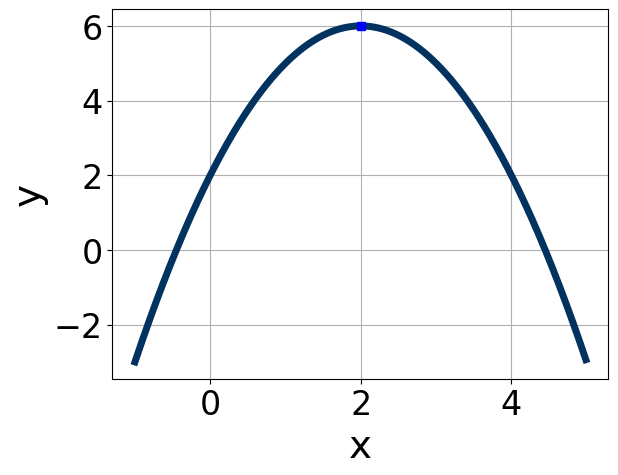
\includegraphics[width=0.5\textwidth]{../Figures/quadraticGraphToEquationCopyB.png}
\end{center}
\begin{enumerate}[label=\Alph*.]
\item \( a \in [-2.8, -0.7], \hspace*{5mm} b \in [-6, -3], \text{ and } \hspace*{5mm} c \in [-11, -9] \)
\item \( a \in [0, 3], \hspace*{5mm} b \in [-6, -3], \text{ and } \hspace*{5mm} c \in [8, 12] \)
\item \( a \in [-2.8, -0.7], \hspace*{5mm} b \in [4, 8], \text{ and } \hspace*{5mm} c \in [1, 3] \)
\item \( a \in [0, 3], \hspace*{5mm} b \in [4, 8], \text{ and } \hspace*{5mm} c \in [8, 12] \)
\item \( a \in [-2.8, -0.7], \hspace*{5mm} b \in [-6, -3], \text{ and } \hspace*{5mm} c \in [1, 3] \)

\end{enumerate} }
\litem{
Factor the quadratic below. Then, choose the intervals that contain the constants in the form $(ax+b)(cx+d); b \leq d.$\[ 36x^{2} +60 x + 25 \]\begin{enumerate}[label=\Alph*.]
\item \( a \in [3.9, 6.6], \hspace*{5mm} b \in [2, 7], \hspace*{5mm} c \in [5.47, 6.34], \text{ and } \hspace*{5mm} d \in [2, 8] \)
\item \( a \in [10.9, 12.9], \hspace*{5mm} b \in [2, 7], \hspace*{5mm} c \in [2.8, 3.1], \text{ and } \hspace*{5mm} d \in [2, 8] \)
\item \( a \in [-0.6, 1.6], \hspace*{5mm} b \in [21, 31], \hspace*{5mm} c \in [0.81, 1.95], \text{ and } \hspace*{5mm} d \in [29, 31] \)
\item \( a \in [1.1, 4.3], \hspace*{5mm} b \in [2, 7], \hspace*{5mm} c \in [9.79, 12.69], \text{ and } \hspace*{5mm} d \in [2, 8] \)
\item \( \text{None of the above.} \)

\end{enumerate} }
\litem{
Solve the quadratic equation below. Then, choose the intervals that the solutions $x_1$ and $x_2$ belong to, with $x_1 \leq x_2$.\[ 10x^{2} -57 x + 54 = 0 \]\begin{enumerate}[label=\Alph*.]
\item \( x_1 \in [0.21, 0.47] \text{ and } x_2 \in [13.33, 14.47] \)
\item \( x_1 \in [1.4, 1.73] \text{ and } x_2 \in [2.3, 3.91] \)
\item \( x_1 \in [0.77, 0.94] \text{ and } x_2 \in [5.55, 7.11] \)
\item \( x_1 \in [1.04, 1.36] \text{ and } x_2 \in [4.17, 5.36] \)
\item \( x_1 \in [11.91, 12.07] \text{ and } x_2 \in [44.83, 45.97] \)

\end{enumerate} }
\litem{
Solve the quadratic equation below. Then, choose the intervals that the solutions belong to, with $x_1 \leq x_2$ (if they exist).\[ 17x^{2} +14 x + 2 = 0 \]\begin{enumerate}[label=\Alph*.]
\item \( x_1 \in [-11.99, -10.69] \text{ and } x_2 \in [-5.1, -3] \)
\item \( x_1 \in [-9.23, -7.19] \text{ and } x_2 \in [7.2, 8.2] \)
\item \( x_1 \in [-0.48, 1.54] \text{ and } x_2 \in [0.3, 1.9] \)
\item \( x_1 \in [-0.93, -0.26] \text{ and } x_2 \in [-0.4, 0.5] \)
\item \( \text{There are no Real solutions.} \)

\end{enumerate} }
\litem{
Factor the quadratic below. Then, choose the intervals that contain the constants in the form $(ax+b)(cx+d); b \leq d.$\[ 24x^{2} -2 x -15 \]\begin{enumerate}[label=\Alph*.]
\item \( a \in [0.3, 2.3], \hspace*{5mm} b \in [-24, -16], \hspace*{5mm} c \in [-0.6, 3.4], \text{ and } \hspace*{5mm} d \in [16, 19] \)
\item \( a \in [2, 3.2], \hspace*{5mm} b \in [-7, -4], \hspace*{5mm} c \in [7.4, 8.3], \text{ and } \hspace*{5mm} d \in [-6, 5] \)
\item \( a \in [17, 21.2], \hspace*{5mm} b \in [-7, -4], \hspace*{5mm} c \in [-0.6, 3.4], \text{ and } \hspace*{5mm} d \in [-6, 5] \)
\item \( a \in [4, 7.3], \hspace*{5mm} b \in [-7, -4], \hspace*{5mm} c \in [3.9, 6.8], \text{ and } \hspace*{5mm} d \in [-6, 5] \)
\item \( \text{None of the above.} \)

\end{enumerate} }
\litem{
Graph the equation below.\[ f(x) = (x+4)^2 + 13 \]\begin{enumerate}[label=\Alph*.]
\begin{multicols}{2}\item 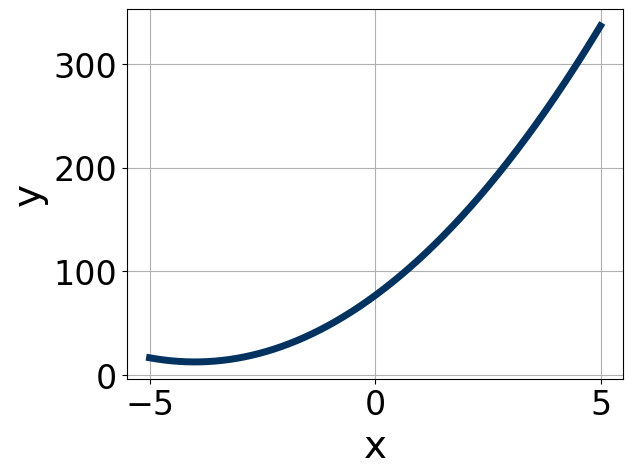
\includegraphics[width = 0.3\textwidth]{../Figures/quadraticEquationToGraphCopyAB.png}\item 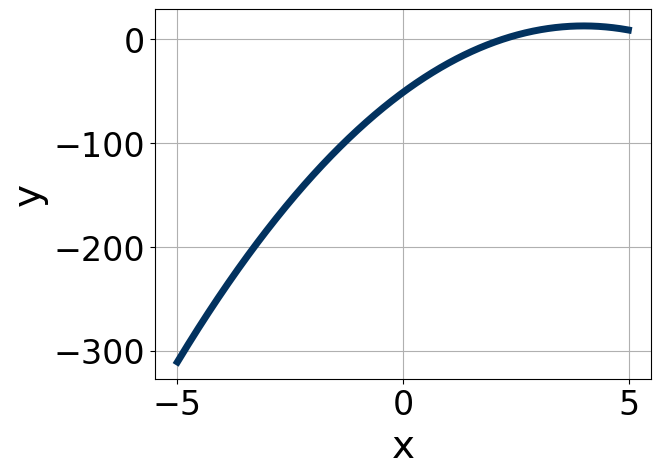
\includegraphics[width = 0.3\textwidth]{../Figures/quadraticEquationToGraphCopyBB.png}\item 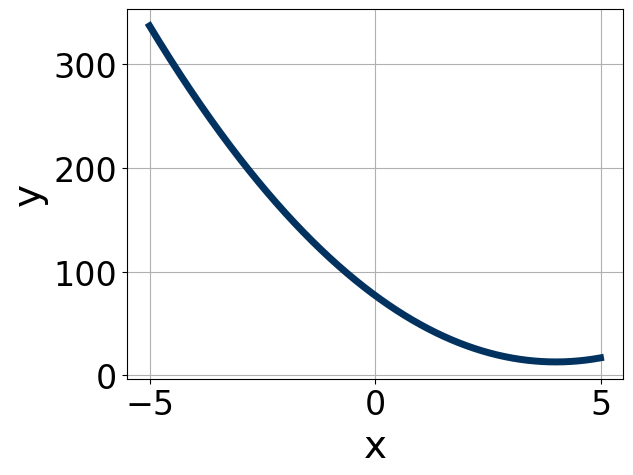
\includegraphics[width = 0.3\textwidth]{../Figures/quadraticEquationToGraphCopyCB.png}\item 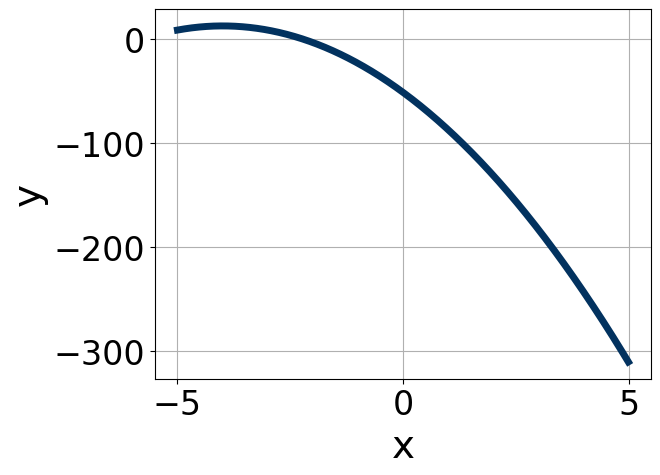
\includegraphics[width = 0.3\textwidth]{../Figures/quadraticEquationToGraphCopyDB.png}\end{multicols}\item None of the above.
\end{enumerate} }
\litem{
Write the equation of the graph presented below in the form $f(x)=ax^2+bx+c$, assuming  $a=1$ or $a=-1$. Then, choose the intervals that $a, b,$ and $c$ belong to.
\begin{center}
    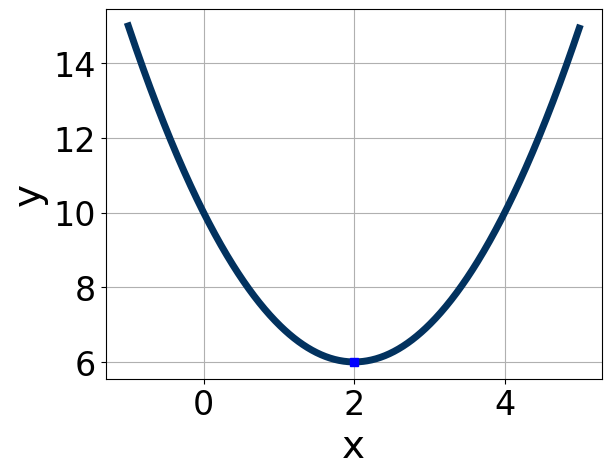
\includegraphics[width=0.5\textwidth]{../Figures/quadraticGraphToEquationB.png}
\end{center}
\begin{enumerate}[label=\Alph*.]
\item \( a \in [0.9, 1.7], \hspace*{5mm} b \in [3, 7], \text{ and } \hspace*{5mm} c \in [8, 11] \)
\item \( a \in [0.9, 1.7], \hspace*{5mm} b \in [3, 7], \text{ and } \hspace*{5mm} c \in [-2, -1] \)
\item \( a \in [-1.2, -0.7], \hspace*{5mm} b \in [3, 7], \text{ and } \hspace*{5mm} c \in [2, 4] \)
\item \( a \in [-1.2, -0.7], \hspace*{5mm} b \in [-4, 0], \text{ and } \hspace*{5mm} c \in [2, 4] \)
\item \( a \in [0.9, 1.7], \hspace*{5mm} b \in [-4, 0], \text{ and } \hspace*{5mm} c \in [8, 11] \)

\end{enumerate} }
\litem{
Graph the equation below.\[ f(x) = -(x-4)^2 - 17 \]\begin{enumerate}[label=\Alph*.]
\begin{multicols}{2}\item 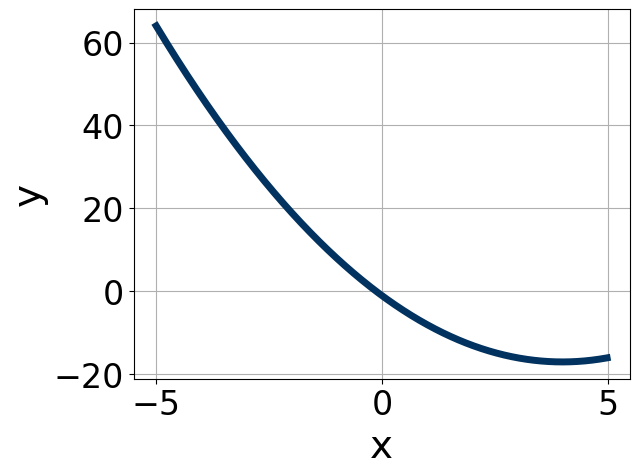
\includegraphics[width = 0.3\textwidth]{../Figures/quadraticEquationToGraphAB.png}\item 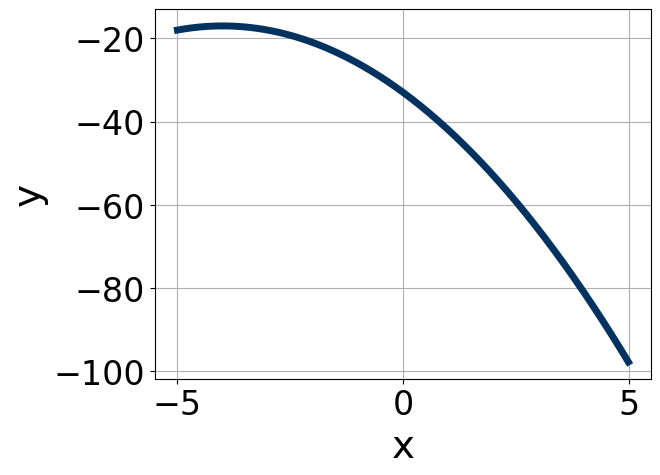
\includegraphics[width = 0.3\textwidth]{../Figures/quadraticEquationToGraphBB.png}\item 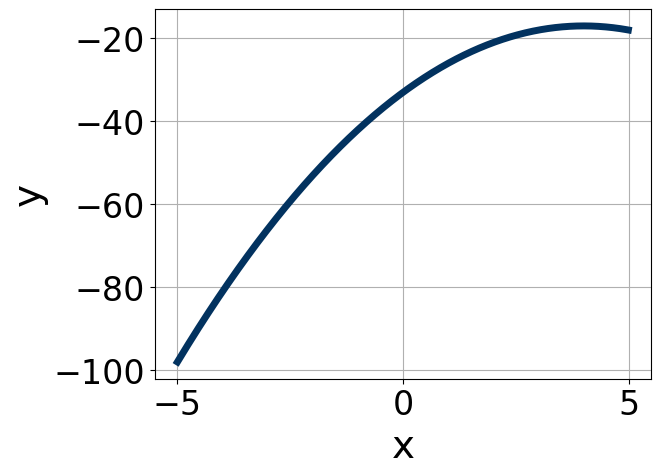
\includegraphics[width = 0.3\textwidth]{../Figures/quadraticEquationToGraphCB.png}\item 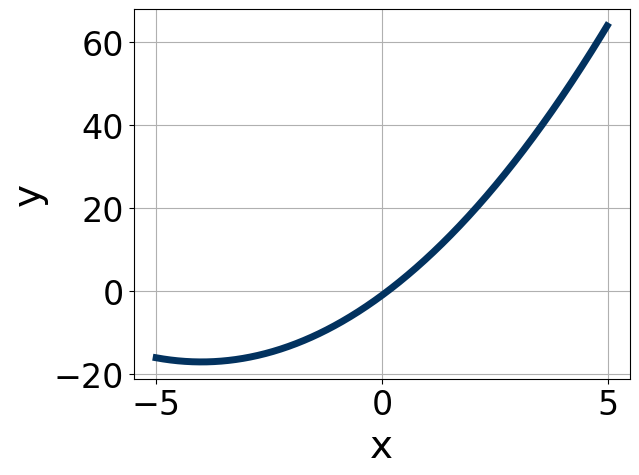
\includegraphics[width = 0.3\textwidth]{../Figures/quadraticEquationToGraphDB.png}\end{multicols}\item None of the above.
\end{enumerate} }
\end{enumerate}

\end{document}